% Graph 7
\documentclass[tikz]{standalone}
\usepackage{tikz}
\usetikzlibrary{bayesnet}

\begin{document}

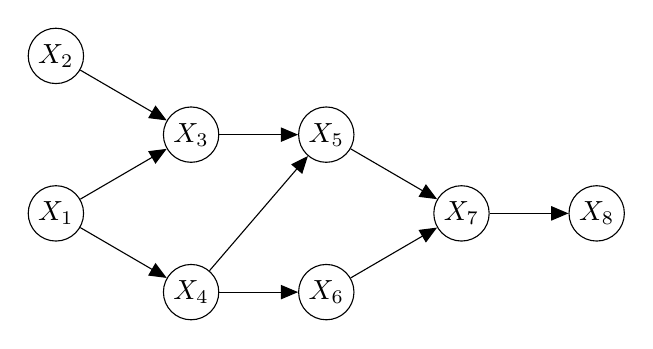
\begin{tikzpicture}
  % Nodes
  \node[latent] (X1) {$X_1$};
  \node[latent, yshift=2cm] (X2) {$X_2$};
  \node[latent, right=of X1, yshift=1.0cm] (X3) {$X_3$};
  \node[latent, right=of X1, yshift=-1.0cm] (X4) {$X_4$};
  \node[latent, right=of X3] (X5) {$X_5$};
  \node[latent, right=of X4] (X6) {$X_6$};
  \node[latent, right=of X5, yshift=-1.0cm] (X7) {$X_7$};
  \node[latent, right=of X7] (X8) {$X_8$};

  % Edges
  \edge {X1} {X3};
  \edge {X2} {X3};
  \edge {X1} {X4};
  \edge {X3} {X5};
  \edge {X4} {X6};
  \edge {X4} {X5};
  \edge {X5} {X7};
  \edge {X6} {X7};
  \edge {X7} {X8};
\end{tikzpicture}

\end{document}